\documentclass[parskip=full]{scrartcl}
\usepackage[utf8]{inputenc}
\usepackage[T1]{fontenc}
\usepackage{graphicx, float}
\graphicspath { {./picture/} }
\usepackage{lmodern}
\usepackage{eurosym}
\usepackage{enumitem}
\usepackage[raggedright]{titlesec}
\usepackage{mathalfa}
\usepackage{titlesec}

\DeclareNewSectionCommands[
style=section,
level=\subparagraphnumdepth+1,
beforeskip=-3.25ex plus -1ex minus -.2ex,
afterskip=1.25ex plus .1ex,
counterwithin=subparagraph,
font={},
indent=0pt,
toclevel=\subparagraphtocdepth+1,
tocnumwidth=6em
]{subsubparagraph,subsubsubparagraph}

\RedeclareSectionCommand[
tocindent=12em
]{subsubparagraph}
\RedeclareSectionCommand[
tocindent=14em
]{subsubsubparagraph}

\RedeclareSectionCommands[
afterskip=1.25ex plus .1ex
]{paragraph,subparagraph}

\setcounter{secnumdepth}{\subsubsubparagraphnumdepth}
\setcounter{tocdepth}{\subsubsubparagraphtocdepth}

\begin{document}
	\begin{titlepage}
		\begin{center}
			\vspace*{1,5cm}
				\textbf{TheArchipelago} \\
			\vspace{0,5cm}
				Written by DragonCoder
			\vspace{1cm}
				\begin{figure}[H]
					\centering
					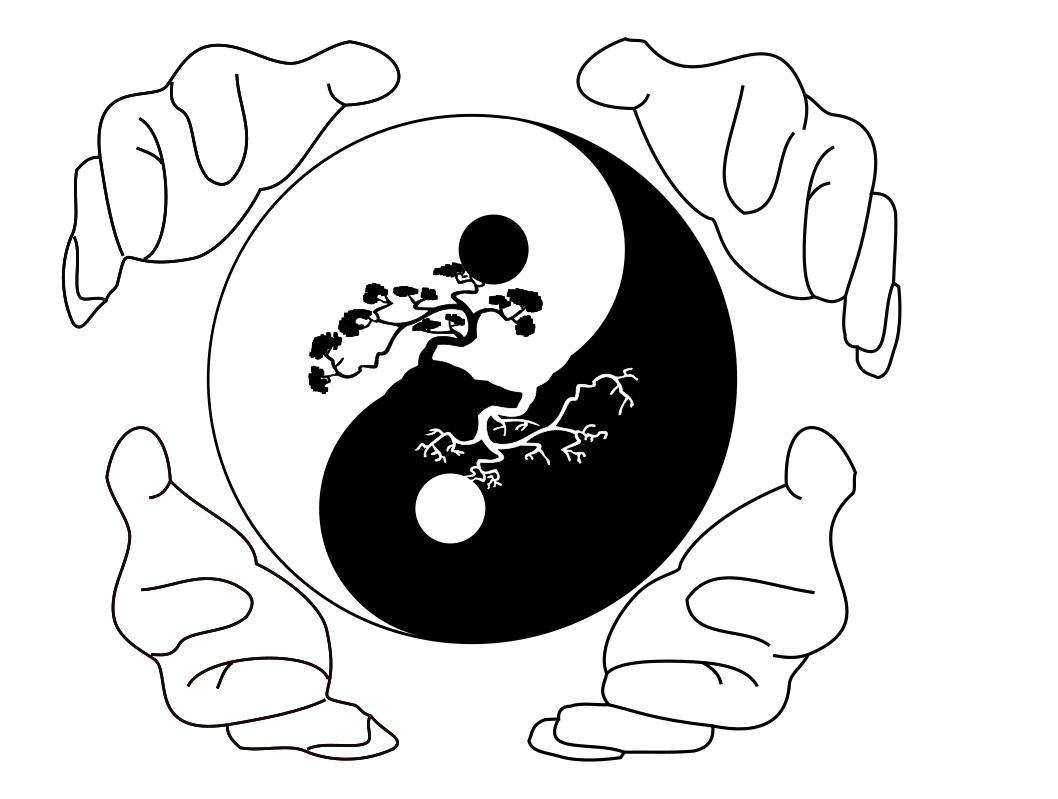
\includegraphics[width=15cm]{logo}
				\end{figure}
		\end{center}
	\end{titlepage}

	\tableofcontents
		\section{Game} \vspace{-5mm}
			\subsection{Game overview} \vspace{-5mm}
				\subsubsection{Motivation} \vspace{-5mm}
					\par \begingroup
					\leftskip=2cm
					\noindent
							The idea for writing a game came in to my head 2 years ago. I searched a game which was interesting, have a nice story, but where is too a PvP motive. I did not find any interesting, then I thought, why not make your own game. I knew, that it not so easy, but I wanted try to do that. First time I have written a easy text game in a console, but I wanted more. I wanted write a game, game on a new level, which no body made, something new in gamedev and I think, that Archipelago can be so one game, when all system will be implemented. Archipelago should be a new generation game, which have not only elements of normal Role Playing Game, but too elements of multiplayer. The game is something like a protest of a new era in the game developing or maybe a shit era for the player and games. Since 2008 it is really hard to find any good games, which give the player a big story, which will really interesting, but has too elements of combat between player 
					\par \endgroup
				\subsubsection{Genre} \vspace{-5mm}
					\par \begingroup
					\leftskip=2cm
					\noindent
							For the begin the game should be a RPG game, but with the time should the game evolve
							to MMO with elements of japan religion. 
					\par \endgroup
				\subsubsection{Target Audience} \vspace{-5mm}
					\par \begingroup
					\leftskip=2cm
					\noindent
							The game shouldn‘t have “special” target audience, the game should be for all people, it isn’t important if there are sink or healthy. I want that all have a possibility to game and I will try to write necessary systems and build a necessary hardware. 
					\par \endgroup
				\subsubsection{Game Flow Summary} \vspace{-5mm}
					\par \begingroup
					\leftskip=2cm
					\noindent
							The Player moves through the game with help of keyboard and in later version with help of extra controller, if he/she will want to use this. The description of the hardware is to find in another part of document. 
					\par \endgroup
				\subsubsection{Look and Feel} \vspace{-5mm}
					\par \begingroup
					\leftskip=2cm
					\noindent
							The basic look should be a 2D look with all religion elements of japan religion and japan map. The player should have a feel like being in the old japan with super hero. It ca be really hard to do without VR, but it will the next idea, next level of the game, next system which should make the game impossible to imitate
					\par \endgroup
				\subsubsection{Project Scope} \vspace{-5mm}
					\paragraph{Number of locations} \vspace{-5mm}
						\par \begingroup
						\leftskip=2cm
						\noindent
								The number of location will be take on with the time. For the version 1.0.0 is planed 2 location, this mean 2 cities.
						\par \endgroup
					\paragraph{Number of levels} \vspace{-5mm}
						\par \begingroup
						\leftskip=2cm
						\noindent
								For the version 1.0.0 is planed 70 levels of character, which will really hard to get, but all level – updates will upper the highest level of character about 10 levels
						\par \endgroup
					\paragraph{Number of NPC’s} \vspace{-5mm}
						\par \begingroup
						\leftskip=2cm
						\noindent
								For the version 1.0.0 will be 3 NPC’s
						\par \endgroup
					\paragraph{Number of weapons} \vspace{-5mm}
						\par \begingroup
						\leftskip=2cm
						\noindent
								For version 1.0.0 will be 5 weapons for one character, but 2 character can use 2 another weapons.
						\par \endgroup
					\paragraph{Number of missions} \vspace{-5mm}
						\par \begingroup
						\leftskip=2cm
						\noindent
								For version 1.0.0 will be 10 missions, but with the update will come next 20
						\par \endgroup
					\paragraph{Number of helmets} \vspace{-5mm}
						\par \begingroup
						\leftskip=2cm
						\noindent	
								For version 1.0.0 will be 8 helmets, which will same for all characters.
						\par \endgroup
					\paragraph{Number of armors} \vspace{-5mm}
						\par \begingroup
						\leftskip=2cm
						\noindent
								For version 1.0.0 will be 20 armors, all another for all character
						\par \endgroup
			\subsection{Gameplay, Mechanics, Mechanisms} \vspace{-5mm}
				\subsubsection{Gameplay} \vspace{-5mm}
					\paragraph{Game Progression} \vspace{-5mm}
						\par \begingroup
						\leftskip=2cm
						\noindent
								The game progression or player progression is a little slow, because of a difficulty of the game, numbers of mission and drop from any bosses. It’s hard to say, how much time the player will need, but the item shop, if any one will be there, will not give a big  protrusion as player, they not use them, because of a game systems. But the progression is so designed that the player has to use or should use the multi-field progression mode in the game, depending on what the character is for.
						\par \endgroup
					\paragraph{Mission/challenge Structure} \vspace{-5mm}
						\par \begingroup
						\leftskip=2cm
						\noindent
								Missions structure is always this same for the version 1.0.0, this mean that the player will become a mission of one NPC and the player have no limited for mostly missions, but with the update will come more time-missions. In the later version of the game  the player will get a possibility to make a own missions, see part with system
						\par \endgroup
					\paragraph{Objectives} \vspace{-5mm}
						\par \begingroup
						\leftskip=2cm
						\noindent
								The objectives of the game is to get all possible items and get the highest level and finished the character of all skills. And most important thing, to have fun. It should be not next game, which will be boring after 2 months and then the player would sell the account.
						\par \endgroup
				\subsubsection{Mechanics and Mechanisms} \vspace{-5mm}
					\paragraph{Physics} \vspace{-5mm}
						\par \begingroup
						\leftskip=2cm
						\noindent
								In this project the physic should be near of reality. The movement of character will be influenced of the map and too rang of the weapon will be near of the reality. For do it possibility in the game will be used ballistics elements for all weapons. 
						\par \endgroup
					\paragraph{Time and season} \vspace{-5mm}
						\par \begingroup
						\leftskip=2cm
						\noindent
								In the game will be implemented normal 24 hours mode and 4 season mode, this mean that one our in the real life is too a one hour in the game from the time zone: UTC +9. The designed of the game will be changed with the seasons.
						\par \endgroup
					\paragraph{Movement} \vspace{-5mm}
						\subparagraph{general movement} \vspace{-5mm}
							\par \begingroup
							\leftskip=2cm
							\noindent
									For the general movement the player will use tasks like [W, A, S, D]
							\par \endgroup
						\subparagraph{other movement} \vspace{-5mm}
							\par \begingroup
							\leftskip=2cm
							\noindent
									As other movement is planed a a controller. But the controller will be not in the first versions of the game. The first controller should be only a prototype and should be only for the hand and make possible to steerage the character movement and usage of skills. In the next versions the controller will be updated to the form of a “overalls”. More about controller:
									\par \begingroup
									\leftskip=2.5cm
									\noindent
											- There will be likely 3 controllers, all will be for the start for no commercial use \\
											- A controller should be responsible for the control of character  and using of accelerometer \\
											- The $2^nd$ controller should be a hand-held keyboard, it mean scarlet that will be put on the hand and has 5 buttons (1 for one finger) \\
											- The $3^rd$ controller is basically the same as the second controller but should be partially used as a mouse with buttons \\
											- Objects Apart from the basic controllers, can be use another small parts, which be connected to the body and will produce a small amount of tension, which should give the player the feeling of being hurt
									\par \endgroup
							\par \endgroup
					\paragraph{Objects} \vspace{-5mm}
						\subparagraph{Picking Up Objects} \vspace{-5mm}
							\par \begingroup
							\leftskip=2cm
							\noindent
									The player will get 30 sec to pick up the item, after 30 sec will the item erase and too the possibility to pick him up.
							\par \endgroup
						\subparagraph{Drop Objects} \vspace{-5mm}
							\par \begingroup
							\leftskip=2cm
							\noindent
									After drop the item has the player 20 sec to pick them up. After 20 sec will the item erase.
							\par \endgroup
						\subparagraph{Moving Objects} \vspace{-5mm}
							\par \begingroup
							\leftskip=2cm
							\noindent
									The items can be moved by using mouse with pick-drop method. The developer will have possibility to move all objects with help of commands.
							\par \endgroup
						\subparagraph{Create objects} \vspace{-5mm}
							\par \begingroup
							\leftskip=2cm
							\noindent
									Only the developer  will have possibility to create any items with help of commands. But it is not this same, like a creating system, it will be to another parts of the game.
							\par \endgroup
						\subparagraph{Coping Objects} \vspace{-5mm}
							\par \begingroup
							\leftskip=2cm
							\noindent
									Only the developer  will have possibility to copy any items with help of commands.
							\par \endgroup
					\paragraph{Actions} \vspace{-5mm}
						\subparagraph{Switches and Buttons} \vspace{-5mm}
							\par \begingroup
							\leftskip=2cm
							\noindent
									In the first version of the game won’t be many buttons or switches. In the version 1.0.0 will be implemented only 3 missions, which will have buttons and NPC’s. For later version the number of buttons will be bigger and to see in missions, interaction with NPC’s, any another systems, user panel etc.
							\par \endgroup
						\subparagraph{Picking Up, Carrying and Dropping} \vspace{-5mm}
							\par \begingroup
							\leftskip=2cm
							\noindent
									Almost all items will be a picking up \& dropping items, this mean that almost all items will can the player drop and picking up, but for later version of the game, all picked items will have name of player whose the item will be. All items will carry by the character in the equipment. 
							\par \endgroup
						\subparagraph{Talking} \vspace{-5mm}
							\par \begingroup
							\leftskip=2cm
							\noindent
									Talking in meaning of Player with Player is to find in point 2.2.10, but talking with the NPC’s or “monster” is planed as a window with buttons, where the player will get mission, but when the player will in a little distance to the NPC, then the player will see and hear, what the NPC will be saying. 
							\par \endgroup
						\subparagraph{Reading} \vspace{-5mm}
							\par \begingroup
							\leftskip=2cm
							\noindent
									Reading as interactions, not only between player and player, but too between player and game world, will be a big system, which should prepare the game to get a new level in the game developing world.
							\par \endgroup
						\subparagraph{Emotions} \vspace{-5mm}
							\par \begingroup
							\leftskip=2cm
							\noindent
									The player will get possibility to show his emotions, but too emotions between 2 players. It isn’t sure if players will have 2 same sex and use partner emotions, because of japan religion.
							\par \endgroup
					\paragraph{Combat} \vspace{-5mm}
						\subparagraph{Player vs Player} \vspace{-5mm}
							\par \begingroup
							\leftskip=2cm
							\noindent
									Player vs Player combat system will be a big system with many possibility to get combat with another player and. By the “last” version of the game will be implemented gambling bet, this mean that the another player can put his money on the another player and so get more many. Behind this idea is too another part of the game, this mean a economy. By the combat players will can choose, if they want fight for money, equipment, range, exp etc.
									\par \begingroup
									\leftskip=2cm
									\noindent
											- 1 vs 1 \\
											- 2 vs 2 \\
											- 5 vs 5 \\
											- death match (all vs all) \\
											- temple vs template \\
									\par \endgroup
							\par \endgroup
						\subparagraph{Player vs Monster} \vspace{-5mm}
							\par \begingroup
							\leftskip=2cm
							\noindent
									Player vs Monster is a normal system, which someone can know from another games, but in the game will be a legendary and antic bosses, which will make the game more interesting and will be part of creating and items upgrade systems. The player will get too a money, exp points, points for passive skills, character skills, equipment etc
							\par \endgroup
					\paragraph{Economy} \vspace{-5mm}
							\par \begingroup
							\leftskip=2cm
							\noindent
									It is not a constant economy of the game because of the players, which will ground the basic of game economy, when the will trade with each other. From developer side will the player get only a special currency. Generally in the game will 3 currencies (version 1.0.0), this mean one of them (Archipelago token) will a normal currency, which the player will use always, when he/she want to buy or to sell something. Another one is more a extension of first one, this means that the Archipelago paper will be like 100 000 of the Archipelago token. The last currency is more a extension of the game, because it will give the player possibility to buy a special items, which will make his/her game a little easier. The game economy will be controlled 24/7 and when the game developer will see, that something is going wrong, then he will take a part in the “refactoring process”.
							\par \endgroup
						\subparagraph{Offline} \vspace{-5mm}
							\par \begingroup
							\leftskip=2cm
							\noindent
									Possibility for player to offline game, but the changes will be only saved in a file, but not on the server/database. The offline mode is too the basic of the all another modes the game.
							\par \endgroup
						\subparagraph{Network} \vspace{-5mm}
							\par \begingroup
							\leftskip=2cm
							\noindent
									Offline mode of the game with possibility to play in a same network.
							\par \endgroup
						\subparagraph{Online} \vspace{-5mm}
							\par \begingroup
							\leftskip=2cm
							\noindent
									The online mode is in principle the main mode of the game and will get more updates as he another modes because of possible to get more bugs.
							\par \endgroup
					\paragraph{Seasons system} \vspace{-5mm}
						\par \begingroup
						\leftskip=2cm
						\noindent
								Some missions will be dependent of the season this mean, that some mission can be finished only in winter this will make the game more interesting and harder to finish the character.
						\par \endgroup
					\paragraph{Chat} \vspace{-5mm}
						\subparagraph{Private} \vspace{-5mm}
							\par \begingroup
							\leftskip=2cm
							\noindent
									In the first versions it will be only a normal chat between 2 player, but for later versions is planed a voice chat between player and something like a messenger, where the player will get the message, which someone sent to him, if the player was offline.
							\par \endgroup
						\subparagraph{Global} \vspace{-5mm}
							\par \begingroup
							\leftskip=2cm
							\noindent
									The global chat will be main chat of the game, where the player will have possibility to buy and sell his items or communicate with all player.
							\par \endgroup
						\subparagraph{Temple} \vspace{-5mm}
							\par \begingroup
							\leftskip=2cm
							\noindent
									Chat only between the temple member.
							\par \endgroup
						\subparagraph{Group} \vspace{-5mm}
							\par \begingroup
							\leftskip=2cm
							\noindent
									Chat only between the group member.
							\par \endgroup
						\subparagraph{Translator} \vspace{-5mm}
							\par \begingroup
							\leftskip=2cm
							\noindent
									Translator should be as a addition for the chat for players which can speak only their languages, but they need to communication with another player.
							\par \endgroup
						\subparagraph{Scanner} \vspace{-5mm}
							\par \begingroup
							\leftskip=2cm
							\noindent
									Scanner is something, what will interfere in personal sphere of all, but this is a important think, which should eliminated racism, possibility to communication and exchange any massages between terrorists, pro right or left groups etc. 
							\par \endgroup
					\paragraph{Make me self} \vspace{-5mm}
						\par \begingroup
						\leftskip=2cm
						\noindent
								“Make me self” system will be once of the important systems which will be implemented in game, not only because of “infinite” development the game, but too as interaction between player – player, player – game developer. In this system player will get possibility to write his own quest, which will be automatically implemented in he game and by the 24h update all player will have 24h to make this quests. The quest needs to be compatible with game story and the prize balanced to complicated level of quest.
						\par \endgroup
					\paragraph{Shops} \vspace{-5mm}
						\par \begingroup
						\leftskip=2cm
						\noindent
								Shops will be only implemented in the online mode of the game \\
						\par \endgroup
						\subparagraph{Offline}
							\par \begingroup
							\leftskip=2cm
							\noindent
									Offline shops should give the player possibility to trade 24/7, but the number of the shops will be limited for eliminate any lags.
							\par \endgroup
						\subparagraph{Online}
							\par \begingroup
							\leftskip=2cm
							\noindent
									Online shops will need, that the player leave the PC on.
							\par \endgroup
					\paragraph{Marriage} \vspace{-5mm}
						\par \begingroup
						\leftskip=2cm
						\noindent
								The marriage will get the two character extra bonuses. On the once side it is hard to implemented marriage between two homosexual because of the religion.
						\par \endgroup
					\paragraph{Range} \vspace{-5mm}
						\par \begingroup
						\leftskip=2cm
						\noindent
								Range system will be something like a extra bonuses system, but the player will get the range points for: combat with players and monster, missions, events. But what is really enjoying that the player can have not only a positive range, but too negative range and this one will make the game harder for the player, then with negative range your all bonus will be 2 times smaller
						\par \endgroup
					\paragraph{Skills} \vspace{-5mm}
						\subparagraph{Character} \vspace{-5mm}
							\par \begingroup
							\leftskip=2cm
							\noindent
									All of the characters get special skills, which are balanced and selected for the character. The character skills can be divided to two parts: buff skills, which make the character stronger and attack skills, which are strengthened by buff skills and make damage. 
							\par \endgroup
						\subparagraph{Passive} \vspace{-5mm}
							\par \begingroup
							\leftskip=2cm
							\noindent
									Passive skills are in 80\% which the player can not upgrade with any training, but skills which the player will upgrade with the time, like “dragon strong”. This skills can the player upgraded only by killing the monster, it is like a range system, but with more levels
							\par \endgroup
					\paragraph{Flowers} \vspace{-5mm}
						\par \begingroup
						\leftskip=2cm
						\noindent
								Flowers as a system is part of more systems. For one as part of crafting system, from the flowers the player will create any potions like strength or sleight potions. For another one as part of mission system and for another one (version 1.0.0) as part of exp system and as temple system.
						\par \endgroup
					\paragraph{Home pets} \vspace{-5mm}
						\par \begingroup
						\leftskip=2cm
						\noindent
								Pets will be most important friend of the character, which will follow the character every where and help him by his new challenge and fighting against troubles. More about the system in another document (“Home pets”).
						\par \endgroup
					\paragraph{Mounts} \vspace{-5mm}
						\par \begingroup
						\leftskip=2cm
						\noindent
								Mounts system is part of moving the character but too combat system. The mounts will help the player to be faster and of getting bigger damage into monster.
						\par \endgroup
					\paragraph{Hazard game} \vspace{-5mm}
						\par \begingroup
						\leftskip=2cm
						\noindent
								Hazard games will be more as entertainment for the player, but too as part of the economic and getting social contacts with another player. All hazard games will base on the old japan/china games with elements of current hazard games. 
						\par \endgroup
					\paragraph{Player shop} \vspace{-5mm}
						\par \begingroup
						\leftskip=2cm
						\noindent
								Player shop is more like a price system. The player get special currency by doing mission, killing monster or another player and then he or she can buy items, which will give their special bonuses, which will make the play in meaning of PvM and PvP system a little easier as players, which will not use this items.
						\par \endgroup
					\paragraph{Stock market} \vspace{-5mm}
						\par \begingroup
						\leftskip=2cm
						\noindent
								The stock market will be part of the economy and as help for player. In the stock market the player will can find minimal and maximal price of items, which will on the shops and the average price. In later version the stock market will get a big update, which will make player life easier.
						\par \endgroup
				\subsubsection{Game Options} \vspace{-5mm}
					\par \begingroup
					\leftskip=2cm
					\noindent
							We or I as developer know, that some people do not have a good graphic card or a good processors, so I want come out to the player and make playing possible for all people, which will want do that. The games options will give possibility all to game in The Archipelago. Most important options like choose between processor and graphic card or uniform look for all all monster, which reduce lags and problems with rendering of monster etc. The player will get too possibility to influence the sound of the game and turns it on and off.
					\par \endgroup
				\subsubsection{Replaying and Saving} \vspace{-5mm}
					\par \begingroup
					\leftskip=2cm
					\noindent
							The replaying and saving of the game is differently of the game mode. When the player will choose online mode, then all records, stats and equipment will be saved in the Data Base, which will get automatically backups all 24 hours. By choosing the network or offline mode will be created files with stats etc, it will be more like a local database.
					\par \endgroup
			\subsection{Story, Setting and Character} \vspace{-5mm}
				\subsubsection{Story} \vspace{-5mm}
					\paragraph{Story} \vspace{-0.5cm}
						\par \begingroup
						\leftskip=2cm
						\noindent
								
						\par \endgroup
					\paragraph{Game Progression} \vspace{-0.5cm}
						\par \begingroup
						\leftskip=2cm
						\noindent
								It really hard to describe the game progression by Archipelago, because of so much possibility to progression of the character. On the one side will the player get possibility to progression his character by PvP mode and on the another hand with PvM mode. Really important fact is, that the player need to use both modes, when he/sie want get all missions and skills. The game progression will be another for player with the 1 lvl and another for someone with 50’s lvl. The player can get a positive or negative progression. Negative progression mean, player lose experience points, when the player is going lose in PvM and PvP. The player will have possibility to prevent the player in his/her progression, this mean bigger rivalry. 
						\par \endgroup
				\subsubsection{Game World} \vspace{-5mm}
					\par \begingroup
					\leftskip=2cm
					\noindent
							All bosses and monsters, which will be respawn on the map, are to finde in another document in form of table.
					\par \endgroup
					\paragraph{General look and feel of world} \vspace{-5mm}
						\par \begingroup
						\leftskip=2cm
						\noindent
								General look of the game will be like more like a fantastic and sweet world with a lot of elements of japan history and their religion. All builds and weapon should be so near of reality as much as possible. But for general position and look of many maps will be used the original map of japan, which should give the player some feeling of reality.
						\par \endgroup
					\paragraph{Shizuoka}\vspace{-0.5cm}
						\subparagraph{General Description} \vspace{-0.5cm}
							\par \begingroup
							\leftskip=2cm
							\noindent
									One of the prefecture in Japan. In the game one of two prefectures, which the player can choose to play there. On the game will be a limit of the shops to relieve the Trade map. The look of the map will be another as by Hamaatsu and some NPC’s will be positioned on the map and the another in Hamaatsu, this mean, that the player need to go from one to another map, when he want get a mission or another one. In the city nobody can’t take part in any battle and hit any players.
							\par \endgroup
						\subparagraph{Physical Characteristics} \vspace{-0.5cm}
							\par \begingroup
							\leftskip=2cm
							\noindent
									Map should look like a little japan city near by water with a circle in center of city, where the NPC's will be
							\par \endgroup
						\subparagraph{Levels that use area} \vspace{-0.5cm}
							\par \begingroup
							\leftskip=2cm
							\noindent
									The player need 1 level of character, which he/she will get by going from birth map and without any maximal level. 
							\par \endgroup
						\subparagraph{Connections to other areas} \vspace{-0.5cm}
							\par \begingroup
							\leftskip=2cm
							\noindent
									The map is connected with another areas through teleporter and with help of Banshin, the God of travel, emigration and immigration. He will teleport the player to any another maps, but first when the player will have min. 15 level of character and need to pay him much money. 
							\par \endgroup
					\paragraph{Hamaatsu}\vspace{-0.5cm}
						\subparagraph{General Description} \vspace{-0.5cm}
							\par \begingroup
							\leftskip=2cm
							\noindent
									One of the prefecture in Japan. In the game one of two prefectures, which the player can choose to play there. On the game will be a limit of the shops to relieve the Trade map. 
							\par \endgroup
						\subparagraph{Physical Characteristics} \vspace{-0.5cm}
							\par \begingroup
							\leftskip=2cm
							\noindent
									Map should look like a little japan city near by water with a circle in center of city, where the NPC's will be
							\par \endgroup
						\subparagraph{Levels that use area} \vspace{-0.5cm}
							\par \begingroup
							\leftskip=2cm
							\noindent
									The player need 1 level of character, which he/she will get by going from birth map and without any maximal level. 
							\par \endgroup
						\subparagraph{Connections to other areas} \vspace{-0.5cm}
							\par \begingroup
							\leftskip=2cm
							\noindent
									The map is connected with another areas through teleporter and with help of Banshin, the God of travel, emigration and immigration. He will teleport the player to any another maps, but first when the player will have min. 15 level of character and need to pay him much money. 
							\par \endgroup
					\paragraph{Trade map}\vspace{-0.5cm}
						\subparagraph{General Description} \vspace{-0.5cm}
							\par \begingroup
							\leftskip=2cm
							\noindent
									Trade map is one of special maps, which is only for trading but not between 2 players, but a place where the player can open a shop with items, which the player want to sell. The map will not have possibility to take any fights between player or to kill/destroy any shop.
							\par \endgroup
						\subparagraph{Physical Characteristics} \vspace{-0.5cm}
							\par \begingroup
							\leftskip=2cm
							\noindent
									- rectangle with circle in middle, where the player can not open shops
									- minimal distance between shops are 5 coordinates
									- limited number of shops \\
									- the character need to have min. 20 lvl to open the shop on the area
							\par \endgroup
						\subparagraph{Levels that use area} \vspace{-0.5cm}
							\par \begingroup
							\leftskip=2cm
							\noindent
									1 lvl to no limit
							\par \endgroup
						\subparagraph{Connections to other areas} \vspace{-0.5cm}
							\par \begingroup
							\leftskip=2cm
							\noindent
									is connected with two cities and the player can be teleport with help of Banshin
							\par \endgroup
					\paragraph{Battle land}\vspace{-0.5cm}
						\subparagraph{General Description} \vspace{-0.5cm}
							\par \begingroup
							\leftskip=2cm
							\noindent
									Battle lands is map for battles between player with much mods. The map will really big, but their will be more parts of the map, which will limited by invisible wall. If it will be any problems, by rendering the map or to big lags, then the Battle land map will be changed to more littler maps.
							\par \endgroup
						\subparagraph{Physical Characteristics} \vspace{-0.5cm}
							\par \begingroup
							\leftskip=2cm
							\noindent
									- Big map \\
									- mixed of maps, this mean a lot elements of another map \\
									- 1 vs 1 area like a little rectangle \\
									- player, who will die more then x times in y time will do teleport to another map \\
									- players with same ip, can't be on the map \\
									- player from one temple can't kill another player from his temple \\
									- limiter, which make it impossible, that player with max level kill someone with 20 lvl or like that
							\par \endgroup
						\subparagraph{Levels that use area} \vspace{-0.5cm}
							\par \begingroup
							\leftskip=2cm
							\noindent
									- 20 level to non limit
							\par \endgroup
						\subparagraph{Connections to other areas} \vspace{-0.5cm}
							\par \begingroup
							\leftskip=2cm
							\noindent
									Only with help of: Ōjina, but the player will be teleport to one of cities
							\par \endgroup
					\paragraph{Birth map}\vspace{-0.5cm}
						\subparagraph{General Description} \vspace{-0.5cm}
							\par \begingroup
							\leftskip=2cm
							\noindent
									Birth map is the first map, which the player will meet on his way. The player will begin his story on the map, while he will search boxes. In the boxes he can find a start equipment like: weapon, armor, which will make the game a little easier. On the map will are 3 boxes and the player can open one of there only 1 time. After opening 3 boxes will the player automatically teleport to one of them prefecture. (The player will get possibility to teleport to the prefecture before he open all boxes).
							\par \endgroup
						\subparagraph{Physical Characteristics} \vspace{-0.5cm}
							\par \begingroup
							\leftskip=2cm
							\noindent
									- middle big map \\
									- constant numbers of boxes \\
									- auto respawn of cases \\
									- auto teleport after opening of all boxes \\
									- impossible to being back there
							\par \endgroup
						\subparagraph{Levels that use area} \vspace{-0.5cm}
							\par \begingroup
							\leftskip=2cm
							\noindent
									The player will be born on the map with 0 lvl 
							\par \endgroup
						\subparagraph{Connections to other areas} \vspace{-0.5cm}
							\par \begingroup
							\leftskip=2cm
							\noindent
									- 
							\par \endgroup
					\paragraph{Mountain pass}\vspace{-0.5cm}
						\subparagraph{General Description} \vspace{-0.5cm}
							\par \begingroup
							\leftskip=2cm
							\noindent
									Mountain pass is map, which should give feeling for the player like “you are in mountain”. This mean, that the player will mostly on the narrow ways. The numbers of way splits is so much, that the player get feel like being in a labyrinth.
							\par \endgroup
						\subparagraph{Physical Characteristics} \vspace{-0.5cm}
							\par \begingroup
							\leftskip=2cm
							\noindent
									- middle big map \\
									- a lot of mountains with some flat places and bigger spots of monsters \\
									- some entries to caves, where the player find extra ores \\
									- snowdrops as extra flowers which are only there to find
							\par \endgroup
						\subparagraph{Levels that use area} \vspace{-0.5cm}
							\par \begingroup
							\leftskip=2cm
							\noindent
									5 level to non maximum, but in later version this possibility will be blocked, that all new player have same possibility to drop and exp. 
							\par \endgroup
						\subparagraph{Connections to other areas} \vspace{-0.5cm}
							\par \begingroup
							\leftskip=2cm
							\noindent
									The map is connected with island of deity and fiery island, and both of cities
							\par \endgroup
					\paragraph{Fiery island}\vspace{-0.5cm}
						\subparagraph{General Description} \vspace{-0.5cm}
							\par \begingroup
							\leftskip=2cm
							\noindent
									Fiery island is one of 4 island of elements, which is focused on fire. The map will like mountain pass, but with littler mountains and in middle of the map will be a big volcano.
							\par \endgroup
						\subparagraph{Physical Characteristics} \vspace{-0.5cm}
							\par \begingroup
							\leftskip=2cm
							\noindent
									- little mountains \\
									- big flames like a column \\
									- special ore and flowers \\
									- little ponds of magma \\
									- big statue of phoenix
							\par \endgroup
						\subparagraph{Levels that use area} \vspace{-0.5cm}
							\par \begingroup
							\leftskip=2cm
							\noindent
									 10 to non limit
							\par \endgroup
						\subparagraph{Connections to other areas} \vspace{-0.5cm}
							\par \begingroup
							\leftskip=2cm
							\noindent
									in the first idea should be the map connection with 3 another islands with a little way or more a tunnel, which look like a part of crystal‑mine.
							\par \endgroup
					\paragraph{Water island}\vspace{-0.5cm}
						\subparagraph{General Description} \vspace{-0.5cm}
							\par \begingroup
							\leftskip=2cm
							\noindent
									Water island will be a island, which will look more like a wetlands. The color of the map will be blue in all possible shadows and green for flowers and trees. 
							\par \endgroup
						\subparagraph{Physical Characteristics} \vspace{-0.5cm}
							\par \begingroup
							\leftskip=2cm
							\noindent
									- look more like the earth under water \\
									- much of a water volcano \\
									- some group of grass \\
									- water holes
							\par \endgroup
						\subparagraph{Levels that use area} \vspace{-0.5cm}
							\par \begingroup
							\leftskip=2cm
							\noindent
									25 level of character to non limit
							\par \endgroup
						\subparagraph{Connections to other areas} \vspace{-0.5cm}
							\par \begingroup
							\leftskip=2cm
							\noindent
									in the first idea should be the map connection with 3 another islands with a little way or more a tunnel, which look like a whirlpool
							\par \endgroup
					\paragraph{Island of the earth}\vspace{-0.5cm}
						\subparagraph{General Description} \vspace{-0.5cm}
							\par \begingroup
							\leftskip=2cm
							\noindent
									Island of the earth is next of the islands. The island should look like a “Big Canyon” with big stones which should look like gods or like a bosses.  On the map will player can find quicksands, which will make the player slower 
							\par \endgroup
						\subparagraph{Physical Characteristics} \vspace{-0.5cm}
							\par \begingroup
							\leftskip=2cm
							\noindent
									- figure of gods or bosses \\
									- big mounts without snow \\
									- quicksand, which make the players slower
							\par \endgroup
						\subparagraph{Levels that use area} \vspace{-0.5cm}
							\par \begingroup
							\leftskip=2cm
							\noindent
									 33 to non limit
							\par \endgroup
						\subparagraph{Connections to other areas} \vspace{-0.5cm}
							\par \begingroup
							\leftskip=2cm
							\noindent
									in the first idea should be the map connection with 3 another islands with a little way or more a tunnel, which look like levitate stones.
							\par \endgroup
					\paragraph{Island of the wind}\vspace{-0.5cm}
							\subparagraph{General Description} \vspace{-0.5cm}
							\par \begingroup
							\leftskip=2cm
							\noindent
									Island of the wind is next of the islands. The most important thing of the map is the storm-look, which should look like a really typhoon and on the map will be some tornados, which will damage the player. But they will respawn in random places and after x second they will change their  position. 
							\par \endgroup
						\subparagraph{Physical Characteristics} \vspace{-0.5cm}
							\par \begingroup
							\leftskip=2cm
							\noindent
									- big map \\
									- random tornados \\
									- more like a w
							\par \endgroup
						\subparagraph{Levels that use area} \vspace{-0.5cm}
							\par \begingroup
							\leftskip=2cm
							\noindent
									45 to non limit
							\par \endgroup
						\subparagraph{Connections to other areas} \vspace{-0.5cm}
							\par \begingroup
							\leftskip=2cm
							\noindent
									in the first idea should be the map connection with 3 another islands with a little way or more a tunnel, which look like a tornado.
							\par \endgroup
					\paragraph{Island of deity}\vspace{-0.5cm}
						\subparagraph{General Description} \vspace{-0.5cm}
							\par \begingroup
							\leftskip=2cm
							\noindent
									Is something another as “Land of the dead”. The monster on this map are more death monster. On this map will are only monster, which look like skeletons.
							\par \endgroup
						\subparagraph{Physical Characteristics} \vspace{-0.5cm}
							\par \begingroup
							\leftskip=2cm
							\noindent
									- Big map \\
									- Map with big walls of bones \\
									- Memorials of bones \\
									- Big skeletons of scorpions \\
									- Bones which hang out from earth  \\
									- dying flowers and trees 
							\par \endgroup
						\subparagraph{Levels that use area} \vspace{-0.5cm}
							\par \begingroup
							\leftskip=2cm
							\noindent
									35 to non limit
							\par \endgroup
						\subparagraph{Connections to other areas} \vspace{-0.5cm}
							\par \begingroup
							\leftskip=2cm
							\noindent
									With help of  Banshin and teleport on mountain pass.
							\par \endgroup
					\paragraph{Land of the dead}\vspace{-0.5cm}
						\subparagraph{General Description} \vspace{-0.5cm}
							\par \begingroup
							\leftskip=2cm
							\noindent
									Land of the dead is a special area, which will be implemented in later version of the game and only for the online mode of the game. The area will not be a normal static area with normal respawn and normal monster, which player can find in another games. On the map will be respawn monsters or more souls of the player which were fallen, this mean, that the number of monster is dependent on number of fallen players.
							\par \endgroup
						\subparagraph{Physical Characteristics} \vspace{-0.5cm}
							\par \begingroup
							\leftskip=2cm
							\noindent
									- big map
									- dynamic respawn of monster with out time limiting
									- only one map with out level limit, where will be possibility to kill another player with out level limit.
									- By getting maximal numbers  of monster on the map, the old monster with lowest level will be destroyed and new monster with higher level will be respawn.
							\par \endgroup
						\subparagraph{Levels that use area} \vspace{-0.5cm}
							\par \begingroup
							\leftskip=2cm
							\noindent
							 		1 to non limit
							\par \endgroup
						\subparagraph{Connections to other areas} \vspace{-0.5cm}
							\par \begingroup
							\leftskip=2cm
							\noindent
									It is only one way. The player need to go to Mountain pass and then to solve a enigma by “Dead Gate” . The number of enigmas will be 10, but with later versions the number of enigmas will grow.
							\par \endgroup
				\subsubsection{Character}\vspace{-0.5cm}
					\paragraph{Hachiman}\vspace{-0.5cm}
						\subparagraph{Background story} \vspace{-0.5cm}
							\par \begingroup
							\leftskip=2cm
							\noindent
									Hachiman is the god of war, who try to protected his county from the monster, who want to kill all of people, who live in Archipelago. Hachiman is very strong and bloodthirsty. Some legends says, that he killed 1000 of death in one battle, but he would hurt and then he is disappear, but now he is coming back. 
							\par \endgroup
						\subparagraph{Look} \vspace{-0.5cm}
							\par \begingroup
							\leftskip=2cm
							\noindent
									- older men \\
									- facial hair \\
									- always dressed like a samurai \\
									- he can use all weapon \\
									- 
							\par \endgroup
						\subparagraph{Special abilities} \vspace{-0.5cm}
							\par \begingroup
							\leftskip=2cm
							\noindent
							
							\par \endgroup
					\paragraph{Jimmu}\vspace{-0.5cm}
						\subparagraph{Background story} \vspace{-0.5cm}
							\par \begingroup
							\leftskip=2cm
							\noindent
							
							\par \endgroup
						\subparagraph{Look} \vspace{-0.5cm}
							\par \begingroup
							\leftskip=2cm
							\noindent
							
							\par \endgroup
						\subparagraph{Special abilities} \vspace{-0.5cm}
							\par \begingroup
							\leftskip=2cm
							\noindent
							
							\par \endgroup
					\paragraph{Senninowie}\vspace{-0.5cm}
						\subparagraph{Background story} \vspace{-0.5cm}
							\par \begingroup
							\leftskip=2cm
							\noindent
							
							\par \endgroup
						\subparagraph{Look} \vspace{-0.5cm}
							\par \begingroup
							\leftskip=2cm
							\noindent
							
							\par \endgroup
						\subparagraph{Special abilities} \vspace{-0.5cm}
							\par \begingroup
							\leftskip=2cm
							\noindent
							
							\par \endgroup
					\paragraph{Susanoo}\vspace{-0.5cm}
						\subparagraph{Background story} \vspace{-0.5cm}
							\par \begingroup
							\leftskip=2cm
							\noindent
							
							\par \endgroup
						\subparagraph{Look} \vspace{-0.5cm}
							\par \begingroup
							\leftskip=2cm
							\noindent
							
							\par \endgroup
						\subparagraph{Special abilities} \vspace{-0.5cm}
							\par \begingroup
							\leftskip=2cm
							\noindent
							
							\par \endgroup
					\paragraph{Tsukuyomi}\vspace{-0.5cm}
						\subparagraph{Background story} \vspace{-0.5cm}
							\par \begingroup
							\leftskip=2cm
							\noindent
							
							\par \endgroup
						\subparagraph{Look} \vspace{-0.5cm}
							\par \begingroup
							\leftskip=2cm
							\noindent
							
							\par \endgroup
						\subparagraph{Special abilities} \vspace{-0.5cm}
							\par \begingroup
							\leftskip=2cm
							\noindent
							
							\par \endgroup
		\section{Controller} \vspace{-5mm}
		\section{App} \vspace{-5mm}
	
	
	
	
	
	
\end{document}